\documentclass[10pt]{article}
\usepackage[margin=0.75in]{geometry}
\usepackage{graphicx}
\usepackage{hyperref}
\setlength{\parindent}{0pt}
\setlength{\parskip}{6pt}
\begin{document}
\section*{n=43 polynomial04: published D4 certificate}
The original independent checker accepted $1\notin W_4(F)$ with codimension at least $2$. A separate exhaustive counter found $2$ ordered Boolean solutions. Since the checked codimension lower bound does not exceed the exact count, this row does not establish last fall degree at least $5$. It certifies degree-four nonmembership for this named Boolean presentation.

\begin{center}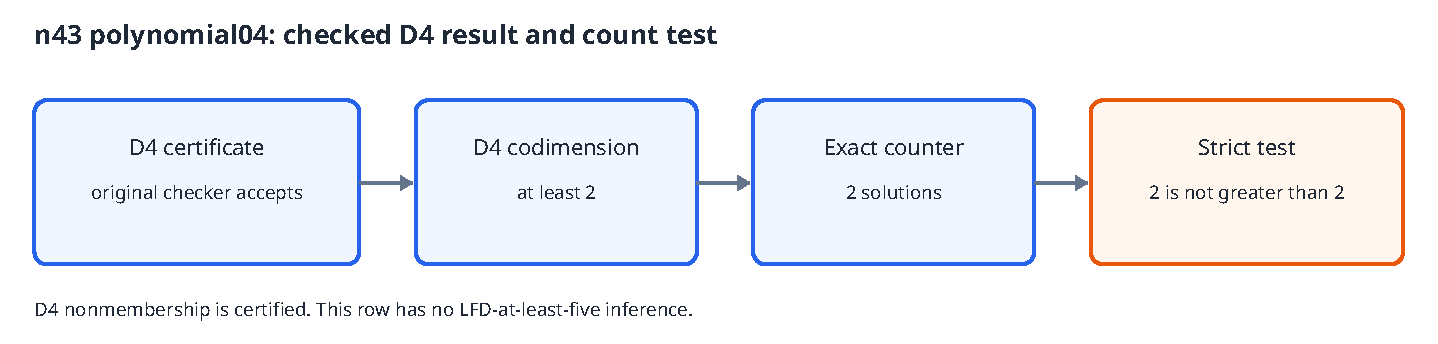
\includegraphics[width=\linewidth]{flow.pdf}\end{center}

\paragraph{Custody.} The retained certificate is 2,399,808 bytes with SHA-256 \texttt{ed165a43...3648d21ae} (full digest in the machine-readable row). The public archive readback verifies anonymous HTTPS and canonical-store downloads of the compressed certificate and evidence bundle and verifies its decompressed bytes. The machine-readable result binds the original result and exact-count inference by SHA-256. The frozen tail continues with subsequent inputs; this report covers this row only.
\end{document}
